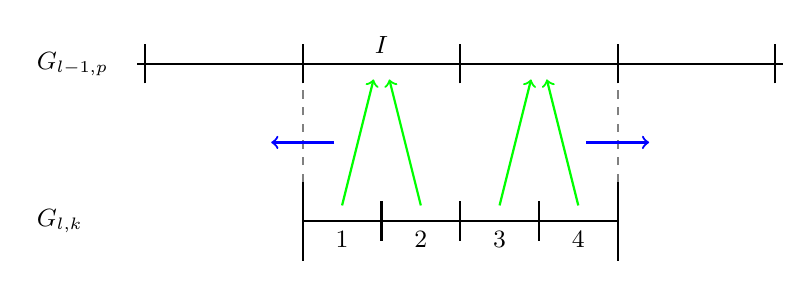
\begin{tikzpicture}
    
   % maillage parent
    
    % ligne horizontale
    \draw[thick] (-0.1, 2) -- (8.1, 2);

    % lignes verticales
    \draw[thick] (0, 1.75) -- (0, 2.25);
    \draw[thick] (8, 1.75) -- (8, 2.25);
    \draw[thick] (2, 1.75) -- (2, 2.25);
    \draw[thick] (4, 1.75) -- (4, 2.25);
    \draw[thick] (6, 1.75) -- (6, 2.25);

    % Annotations
    \node[right] at (-1.5, 2) {\small \(G_{l-1, p}\)};
    \node[above] at (3, 2) {\small \(I\)};

    % maillage secondaire

    % ligne horizontale    
    \draw[thick] (2, 0) -- (6, 0);

    % lignes verticales
    \draw[thick] (2, -0.5) -- (2, 0.5);
    \draw[thick] (6, -0.5) -- (6, 0.5);
    \draw[thick] (3, -0.25) -- (3, 0.25);
    \draw[thick] (4, -0.25) -- (4, 0.25);
    \draw[thick] (5, -0.25) -- (5, 0.25);

    % Annotations
    \node[right] at (-1.5, 0) {\small \( G_{l, k} \)};
    \node[below] at (2.5, 0) {\small \(1\)};
    \node[below] at (3.5, 0) {\small \(2\)};
    \node[below] at (4.5, 0) {\small \(3\)};
    \node[below] at (5.5, 0) {\small \(4\)};

    % liaisons entre maillage
    \draw[dashed, thick, gray] (2, 0.5) -- (2, 1.75);
    \draw[dashed, thick, gray] (6, 0.5) -- (6, 1.75);

    % Correction des mailles raffinées
    \draw[->, thick, green] (2.5, 0.2) -- (2.9, 1.8);
    \draw[->, thick, green] (3.5, 0.2) -- (3.1, 1.8);
    \draw[->, thick, green] (4.5, 0.2) -- (4.9, 1.8);
    \draw[->, thick, green] (5.5, 0.2) -- (5.1, 1.8);

    % Correction des flux
    \draw[->, thick, blue] (2.4, 1) -- (1.6, 1);
    \draw[->, thick, blue] (5.6, 1) -- (6.4, 1);
\end{tikzpicture}